\par DFT và các biến đổi mang ý nghĩa tương đương khi biến đổi miền không gian sang miền tần số được ứng dụng trong việc nén ảnh số có và không mất mát thông tin mà trong đó, hiện nay ứng dụng rộng rãi nhất đó là kĩ thuật nén ảnh số JPEG. Các nghiên cứu về nén ảnh số xoay quanh vấn đề giảm thiểu dung lượng file ảnh gốc tuy nhiên vẫn giữ được chất lượng mà mắt con người vẫn có thể nhận biết rõ ràng. Đồ án sẽ xây dựng chương trình nén ảnh số dựa trên bài báo [15].
\section{Kĩ thuật đường ống}
Kĩ thuật đường ống của chương trình nén ảnh được thể hiện qua sơ đồ sau:
\begin{center}
    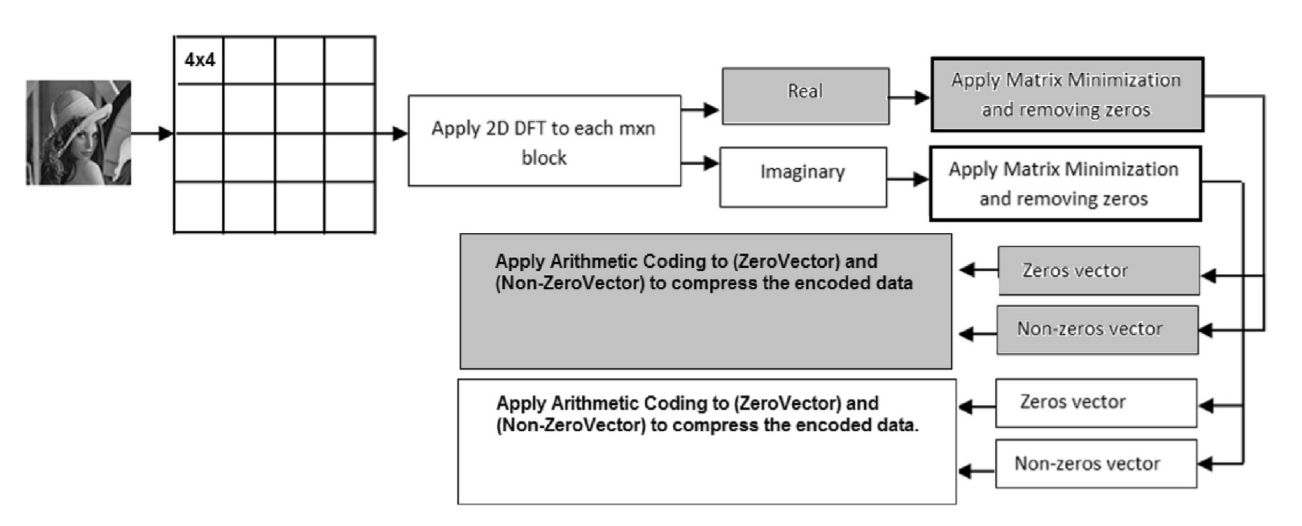
\includegraphics[scale=0.5]{Figures/fig17.png}
    \par \textbf {Hình 3.1} Phương án đề xuất [15].
\end{center}
\par Kĩ thuật nén ảnh được xây dựng dựa trên cơ sở ảnh đầu vào là ảnh xám, đối với ảnh màu có thể coi mỗi kênh màu là một ảnh xám và thực hiện nén trên từng kênh. Kết quả thu được sẽ được nối lại theo thứ tự. Mỗi bức ảnh xám ban đầu sẽ được thực hiện theo các bước như sau:
\subsection{Áp dụng DFT trên từng khối}
\par Việc thực hiện DFT trên từng khối, mặc định là khối có kích thước 4x4 sẽ đưa mỗi khối của ảnh gốc ban đầu từ miền không gian sang miền tần số. Giống như đã trình bày ở phần lọc ảnh, giá trị đầu tiên của mỗi khối là giá trị tần số thấp sẽ mang đặc trưng liên quan đến chi tiết, hình dạng của vật thể trong ảnh, sẽ được trích xuất ra một vector riêng và được bảo toàn nhằm giữ lại chất lượng hình ảnh một cách tốt nhất. Vector này được gọi là LFC (Low-Frequency-Components). Ma trận còn lại sau khi loại bỏ LFC được gọi là ma trận HFC (High-Frequency-Components) khi chỉ mang những giá trị tần số cao.

\begin{itemize}
    \item Nén: Thông qua ảnh ban đầu và biến đổi DFT trên từng khối trích xuất ma trận LFC và HFC.
    \item Giải nén: Từ vector LFC và HFC kết hợp với biến đổi IDFT trên từng khối thu được ảnh đã được giải nén. 
\end{itemize}

\begin{center}
    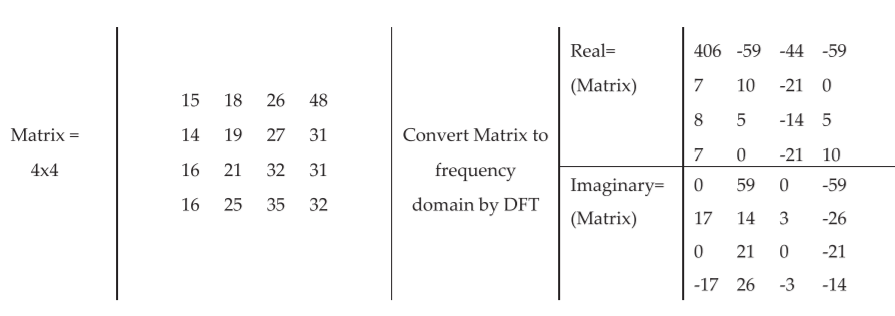
\includegraphics[scale=0.65]{Figures/fig18.png}
    \par \textbf {Hình 3.2} Biến đổi DFT trên từng khối [15].
\end{center}
\subsection{Lượng tử hóa}
\par Kĩ thuật lượng tử hóa (quantization) thường được sử dụng trong các phương pháp nén có mất mát dữ liệu. Các giá trị của vector hoặc ma trận sẽ được chia cho giá trị $q$ (ví dụ $q=20$) và được làm tròn đến số nguyên gần nhất. Quá trình giải nén dữ liệu sẽ được nhân với giá trị $q$ ban đầu.
\begin{center}
    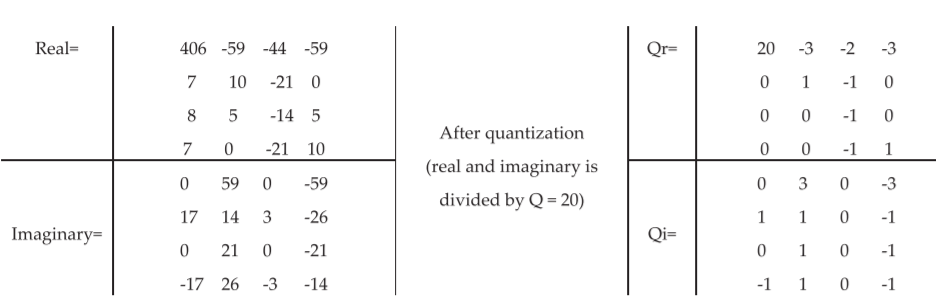
\includegraphics[scale=0.6]{Figures/fig19.png}
    \par \textbf {Hình 3.3} Quá trình lượng tử hóa [15].
\end{center}
\subsection{Áp dụng thuật toán Matrix Minimization [15]}
\par Thông qua việc trích xuất vector LFC và ma trận HFC và lượng tử hóa. Dễ thấy rằng kích thước LFC nhỏ hơn 16 lần (đối với khối có kích thước 4x4) so với kích thước HFC. Do vậy, ta cần phải nén ma trận HFC. Việc này được thực hiện bằng thuật toán Matrix Minimization [15].
\par Thuật toán sinh ngẫu nhiên 3 giá trị, thường nằm trong khoảng $(0, 1)$, thực hiện nhân với các khối không chồng lên nhau và cộng lấy giá trị cuối. Như vậy kích thước của vector đầu ra giảm 3 lần so với ban đầu. Khóa K và bảng giá trị Limited-data được lưu lại cho quá trình giải nén. Thuật toán giải nén được sử dụng là tìm kiếm tuần tự (Linear Sequential Search) tuy đơn giản nhưng chi phí tính toán cao.
\begin{itemize}
    \item Nén: thuật toán Matrix Minimization.
    \item Giải nén: thuật toán tìm kiếm tuần tự.
\end{itemize}

\begin{center}
    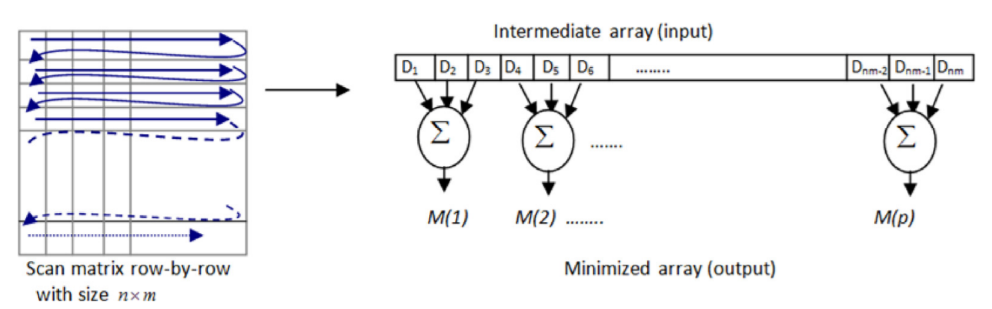
\includegraphics[scale=0.6]{Figures/fig21.png}
    \par \textbf {Hình 3.4} Thuật toán Matrix Minimization [15].
\end{center}
\begin{algorithm}[H]
%\SetAlgoLined
\textbf{Input: } Ma trận HFC.\\
\textbf{Output: } Ma trận HFC đã được tối thiểu hóa.\\
\textbf{function } HFC\_minimized $\leftarrow$ $MM$(HFC):\\
\hspace{10mm} \# Tạo 3 giá trị khóa ngẫu nhiên trong khoảng (0, 1)\\
\hspace{10mm} K = rand(1, 3)\\
\hspace{10mm} \# Duỗi thẳng ma trận HFC\\
\hspace{10mm} [height, width] $\leftarrow$ size(HFC)\\
\hspace{10mm} tmp $\leftarrow$ 1\\
\hspace{10mm} for i = 1 to height do\\
\hspace{20mm} for j = 1 to width do\\
\hspace{30mm} HFC\_flatted(tmp) $\leftarrow$ HFC(i, j)\\
\hspace{30mm} tmp $\leftarrow$ tmp + 1\\
\hspace{20mm} endfor\\
\hspace{10mm} endfor\\
\hspace{10mm} \# Lặp\\
\hspace{10mm} tmp $\leftarrow$ 1\\
\hspace{10mm} j $\leftarrow$ 1\\
\hspace{10mm} while (j < height * width) do\\
\hspace{20mm} sum $\leftarrow$ HFC\_flatted(j)*K(1) + HFC\_flatted(j+1)*K(2) + HFC\_flatted(j+2)*K(3) \\
\hspace{20mm} HFC\_minimized(tmp) $\leftarrow$ sum\\
\hspace{20mm} tmp $\leftarrow$ tmp + 1\\
\hspace{20mm} j $\leftarrow$ j + 3\\
\hspace{10mm} end\\
 \caption{Thuật toán Matrix Minimization Encoding}
\end{algorithm}


\subsection{Thuật toán Aritmetic Coding [15]}
\par Khái niệm entropy dùng để chỉ mức độ hỗn loạn của thông tin. Với một thông tin $x$ có thể nhận các giá trị $i$ với xác suất $p(i)$, entropy (kí hiệu là $S$) được định nghĩa theo công thức:
$$S =  - \sum\limits_i {p(i)\log (p(i))}.$$
\par Aritmetic Coding (AC) là thuật toán nén dữ liệu dựa trên lý thuyết thông tin, cho phép lưu trữ thông tin với số lượng bits tối thiểu. Claude Shannon chỉ ra rằng không thể nào lưu trữ thông tin với số bits nhỏ hơn entropy của thông tin này. AC cho phép tiến tới gần giới hạn entropy này với khoảng cách 2 bits.
\par Để đảm bảo hiệu quả cho thuật toán Aritmetic Coding, khi mà số lượng các giá trị 0 chiếm số lượng lớn trong dữ liệu, ta thực hiện việc tách vector HFC ban đầu thành 2 vector con định nghĩa phần giá trị khác 0 và giá trị bằng 0 (hình 3.5) và thực hiện mã hóa Aritmetic. 
\begin{center}
    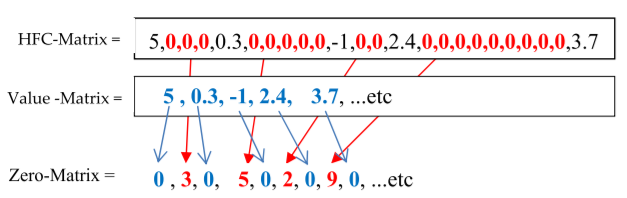
\includegraphics[scale=0.8]{Figures/fig22.png}
    \par \textbf {Hình 3.5} Tách vector HFC thành vector 0 và vector giá trị [15].
\end{center}
\section{Quá trình giải mã}
\par Quá trình giải nén được thực hiện tuần tự theo chiều ngược lại của quá trình nén, các bước như sau:
\begin{itemize}
    \item Áp dụng thuật toán giải nén Aritmetic Decoding.
    \item Kết hợp các vector 0 và vector giá trị để thu được vector HFC đã được tối thiểu và vector LFC.
    \item Thuật toán giải nén Matrix Minimization Decoding cho vector HFC tối thiểu để thu được vector HFC.
    \item Kết hợp vector HFC và vector LFC và thực hiện IDFT trên từng khối để thu được ảnh đã giải nén.
\end{itemize}
\par Quá trình giải nén được thể hiện qua sơ đồ sau:
\begin{center}
    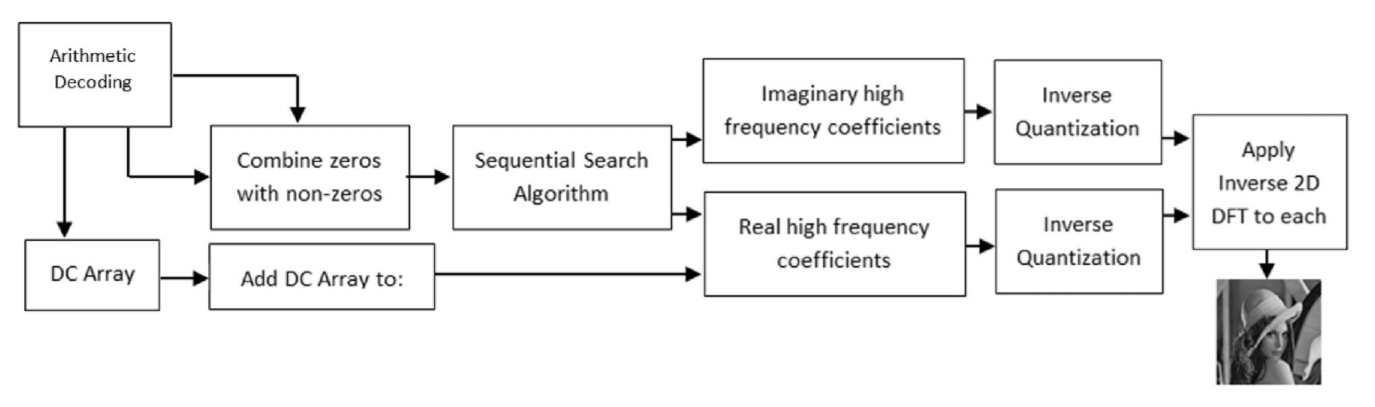
\includegraphics[scale=0.45]{Figures/fig23.png}
    \par \textbf {Hình 3.6} Sơ đồ giải nén ảnh [15].
\end{center}
\section{Kết quả}
\par Sự chênh lệch giữa ảnh gốc và ảnh đã nén và giải nén được đánh giá qua tiêu chuẩn RMSE:
$$RMSE(y, y') = \sqrt {\frac{{\sum\limits_{i = 1}^H {\sum\limits_{j = 1}^W {\sum\limits_{k = 1}^C {{{(y(i,j,k) - y'(i,j,k))}^2}} } } }}{{H.W.C}}}$$
với $y, y'$ lần lượt là ma trận ảnh gốc và ảnh sau khi giải nén, $H, W, C$ lần lượt là chiều rộng, chiều dài và số kênh màu của ảnh.
\par Thuật toán hoạt động khá tốt, nhưng gặp phải một số hạn chế nhất định như giá trị lượng tử hóa q được lựa chọn một cách heuristic [15] và những giá trị cao không thể hoạt động tốt trong tất cả các trường hợp. Ví dụ như giá trị lượng tử hóa cao vẫn giúp giữ lại chất lượng ảnh tốt cho dù định dạng TIF hay PNG và ảnh màu hay ảnh xám (hình 3.8, hình 3.9, hình 3.10), nhưng lại gây ra hiện tượng thay đổi rõ rệt chất lượng trong một số ảnh, đặc biệt là ảnh kích thước nhỏ (hình 3.7, hình 3.11). Và bên cạnh việc quá trình nén ảnh không tốn nhiều tài nguyên nhưng quá trình giải nén ảnh tốn khá nhiều tài nguyên và thời gian, chủ yếu ở thuật toán tìm kiếm tuần tự.
\par Kết quả của thuật toán nén ảnh được mô tả qua bảng 3.1.
\vspace{10mm}
\begin{center}
\begin{tabular}{|c|c|c|c|c|l|}
\hline
\multirow{2}{*}{Ảnh} & \multirow{2}{*}{\begin{tabular}[c]{@{}c@{}}Kích thước\\ 8-bits (kB)\end{tabular}} & \multirow{2}{*}{\begin{tabular}[c]{@{}c@{}}Kích thước \\ file (kB)\end{tabular}} & \multirow{2}{*}{q} & \multirow{2}{*}{\begin{tabular}[c]{@{}c@{}}Kích thước\\ nén (kB)\end{tabular}} & \multicolumn{1}{c|}{\multirow{2}{*}{RMSE}} \\
 &  &  &  &  & \multicolumn{1}{c|}{} \\ \hline
\multirow{3}{*}{\begin{tabular}[c]{@{}c@{}}lena.tif\\ (512x512)\end{tabular}} & \multirow{3}{*}{\begin{tabular}[c]{@{}c@{}}768\\ (color)\end{tabular}} & \multirow{3}{*}{768} & 10 & 614 & 1.9495 \\ \cline{4-6} 
 &  &  & 20 & 421 & 2.8530 \\ \cline{4-6} 
 &  &  & 40 & 253 & 24.2674 \\ \hline
\multirow{3}{*}{\begin{tabular}[c]{@{}c@{}}airplane.png\\ (512x512)\end{tabular}} & \multirow{3}{*}{\begin{tabular}[c]{@{}c@{}}768\\ (color)\end{tabular}} & \multirow{3}{*}{439} & 20 & 362 & 2.3843 \\ \cline{4-6} 
 &  &  & 40 & 213 & 5.5639 \\ \cline{4-6} 
 &  &  & 60 & 154 & 8.7267 \\ \hline
\multirow{3}{*}{\begin{tabular}[c]{@{}c@{}}pepers.png\\ (512x512)\end{tabular}} & \multirow{3}{*}{\begin{tabular}[c]{@{}c@{}}768\\ (color)\end{tabular}} & \multirow{3}{*}{526} & 20 & 451 & 4.2847 \\ \cline{4-6} 
 &  &  & 40 & 273 & 7.3025 \\ \cline{4-6} 
 &  &  & 60 & 184 & 9.8472 \\ \hline
\multirow{3}{*}{\begin{tabular}[c]{@{}c@{}}cameraman.tif\\ (256x256)\end{tabular}} & \multirow{3}{*}{\begin{tabular}[c]{@{}c@{}}65.5\\ (gray)\end{tabular}} & \multirow{3}{*}{63.7} & 10 & 52.2 & 1.5214 \\ \cline{4-6} 
 &  &  & 40 & 23.8 & 5.9341 \\ \cline{4-6} 
 &  &  & 80 & 15.5 & 10.9548 \\ \hline
\end{tabular}
\end{center}
\begin{center}
\par Bảng 3.1: Kết quả thuật toán nén ảnh.
\end{center}
\begin{center}
    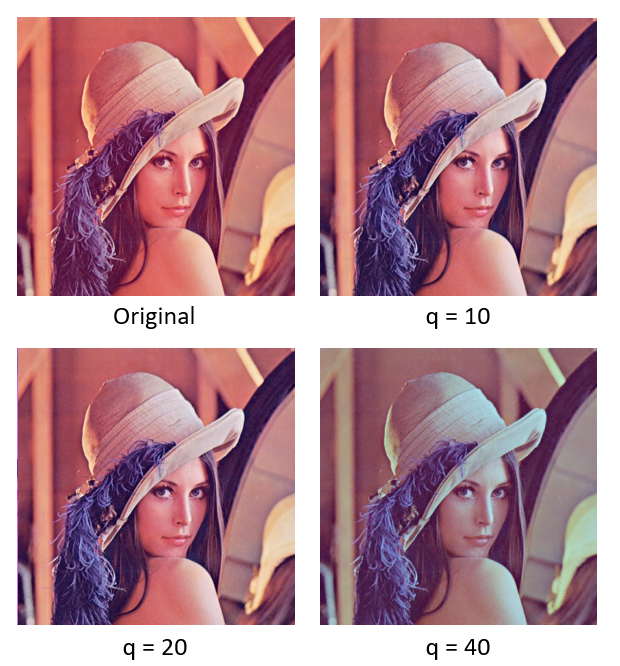
\includegraphics[scale=0.53]{Figures/fig27.png}
    \par \textbf {Hình 3.7} Kết quả nén ảnh lena.tif.
\end{center}
\begin{center}
    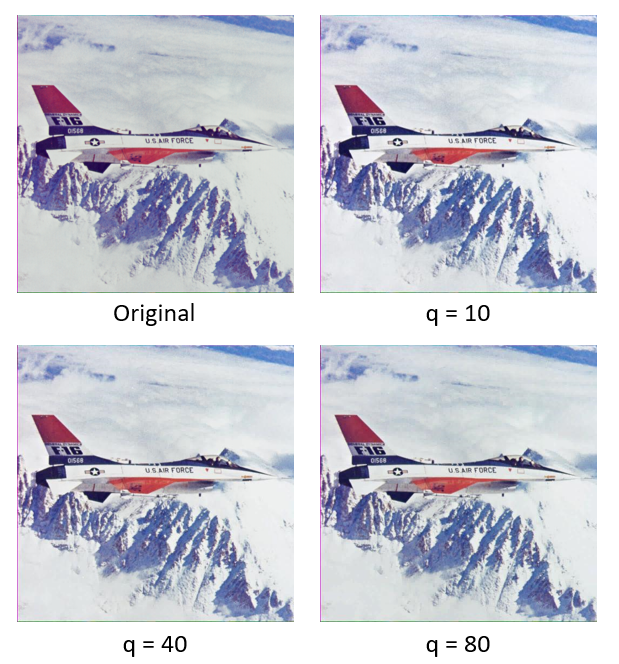
\includegraphics[scale=0.53]{Figures/fig26.png}
    \par \textbf {Hình 3.8} Kết quả nén ảnh airplane.png.
\end{center}
\begin{center}
    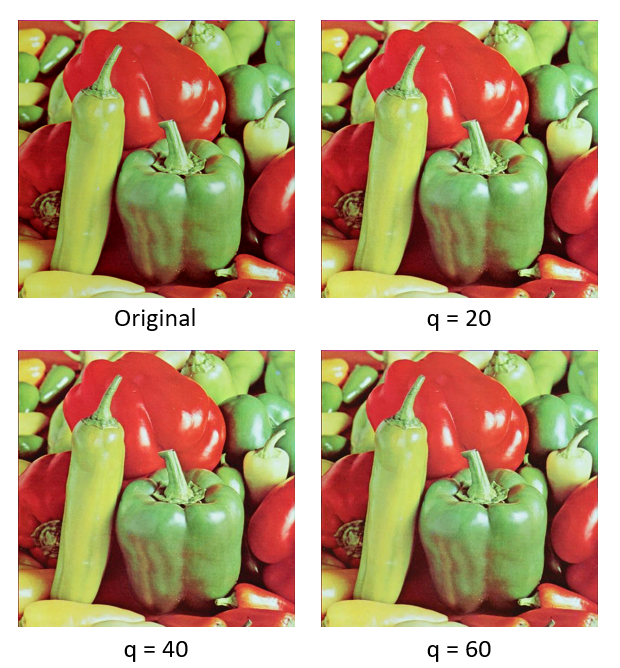
\includegraphics[scale=0.53]{Figures/fig28.png}
    \par \textbf {Hình 3.9} Kết quả nén ảnh pepers.png.
\end{center}
\begin{center}
    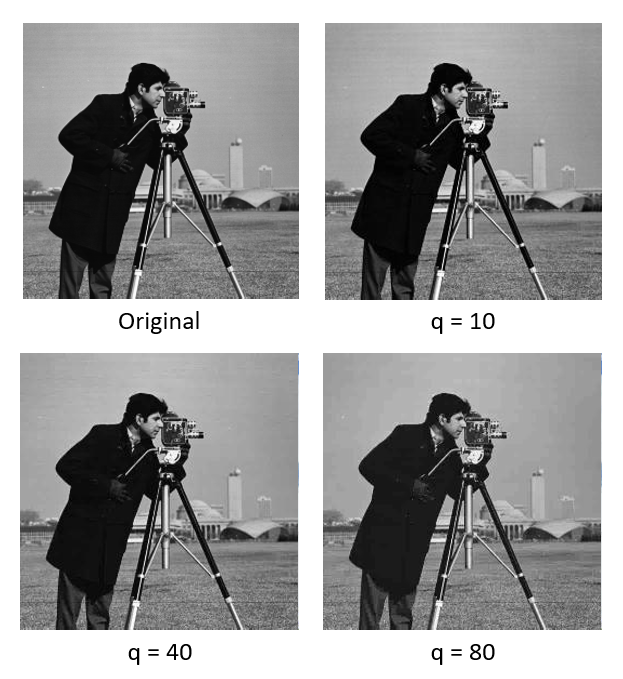
\includegraphics[scale=0.53]{Figures/fig25.png}
    \par \textbf {Hình 3.10} Kết quả nén ảnh cameraman.tif.
\end{center}
\begin{center}
    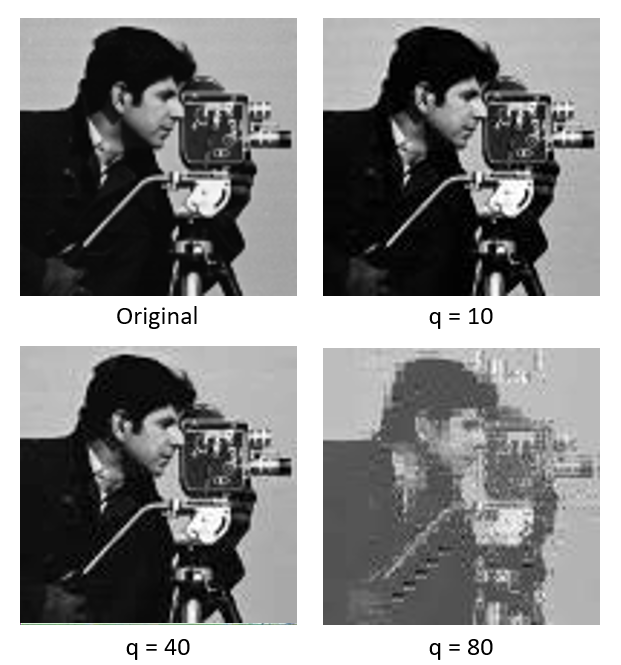
\includegraphics[scale=0.53]{Figures/fig29.png}
    \par \textbf {Hình 3.11} Kết quả nén một phần ảnh cameraman.tif kích thước 96x96.
\end{center}